\setchapterpreamble[u]{\margintoc}
\chapter{Контекстно-свободные языки в качестве ограничения на пути}
\label{chpt:CFPQ}
\tikzsetfigurename{CFPQ_}

\mytodo{Добавить во введение: обзор структуры главы, связь с секцией 5 главы 10}

В данной главе мы рассмотрим алгоритмы поиска путей с контекстно-свободными ограничениями в графах. Эти алгоритмы обобщают классические методы синтаксического анализа (глава~\ref{chpt:ClassicalParsing}) на случай графов, заменяя позиции в строке на вершины графа.

Задача КС-достижимости была впервые сформулирована Михалисом Яннакакисом в 1990~году~\sidecite{Yannakakis}.
С тех пор было предложено множество алгоритмов: на основе CYK (Хеллингс~\sidecite{hellingsPathQuerying,hellingsRelational,DBLP:journals/corr/Hellings15}), на основе (G)LL и (G)LR (Медейрос и~др.~\sidecite{MEDEIROS201975}, Сантос и~др.~\sidecite{10.1007/978-3-319-91662-0_17}, Григорьев и~др.~\sidecite{Grigorev:2017:CPQ:3166094.3166104}, Вербицкая и~др.~\sidecite{10.1007/978-3-319-41579-6_22}), на основе матричных операций (Азимов~\sidecite{Azimov:2018:CPQ:3210259.3210264}, Терехов и~др.~\sidecite{Terekhov2021MultipleSourceCP}), а также подход на основе комбинаторов парсеров (Вербицкая и~др.~\sidecite{Verbitskaia:2018:PCC:3241653.3241655}).
Экспериментальное исследование Кёйперса и~др.~\sidecite{Kuijpers:2019:ESC:3335783.3335791} показало, что производительность многих алгоритмов на реальных данных остаётся недостаточной; матричные алгоритмы, использующие высокопроизводительные библиотеки линейной алгебры, демонстрируют лучшие результаты (Мишин и~др.~\sidecite{Mishin:2019:ECP:3327964.3328503}, Терехов и~др.~\sidecite{10.1145/3398682.3399163}).

\input{part_03_GraphAnalysis/chapter_12_CFPQ/01_Hellings}
\section[Алгоритмы на основе произведения матриц для всех пар вершин]{Алгоритмы на основе произведения матриц для всех пар вершин}
	\tikzsetfigurename{CFPQ_MatrixBased_}
\sectionmark{Алгоритмы на основе произведения матриц для всех пар вершин}
	\tikzsetfigurename{CFPQ_MatrixBased_}
\label{sec:CFPQ_MatrixBased}

В разделе~\ref{sec:CFPQ_Hellings}~был изложен алгоритм для решения задачи КС достижимости на основе CYK.
Заметим, что обход матрицы напоминает умножение матриц в ячейках которых множества нетерминалов:
\begin{align*}
M_3 = &M_1 \times M_2 \\
M_3[i,j] = &\sum_{k=1}^{n} M[i,k] * M[k,j]
\end{align*}
, где сумма~--- это объединение множеств:
\[
\sum_{k=1}^{n} = \bigcup_{k=1}^{n}
\]
, а поэлементное умножение определено следующим образом:
\[
S_1 * S_2 = \{N_1^0 ... N_1^m\} * \{N_2^0 ... N_2^l\} = \{N_3 \mid (N_3 \rightarrow N_1^i N_2^j) \in P\}.
\]
Таким образом, алгоритм решения задачи КС достижимости может быть выражена в терминах перемножения матриц над полукольцом с соответствующими операциями.

Для частного случая этой задачи, синтаксического анализа линейного входа, существует алгоритм Валианта~\cite{Valiant:1975:GCR:1739932.1740048}, использующий эту идею.
Однако он не обобщается на графы из-за того, что существенно использует возможность упорядочить обход матрицы (см. разницу в CYK для линейного случая и для графа).
Поэтому, хотя для линейного случая алгоритм Валианта является алгоритмом синтаксического анализа для произвольных КС грамматик за субкубическое время, его обобщение до задачи КС достижимости в произвольных графах с сохранением асимптотики является нетривиальной задачей~\cite{Yannakakis}.
В настоящее время алгоритм с субкубической сложностью получен только для частного случая~--- языка Дика с одним типом скобок~--- Филипом Брэдфордом~\cite{8249039}.

В случае с линейным входом, отдельного внимания заслуживает работа Лиллиан Ли (Lillian Lee)~\cite{Lee:2002:FCG:505241.505242}, где она показывает, что задача перемножения матриц сводима к синтаксическому анализу линейного входа. Аналогичных результатов для графов на текущий момент не известно.

Поэтому рассмотрим более простую идею, изложенную в статье Рустама Азимова~\cite{Azimov:2018:CPQ:3210259.3210264}: будем строить транзитивное замыкание графа через наивное (не через возведение в квадрат) умножение матриц.

Пусть $\mathcal{G} = (V, E)$~--- входной граф и $G = (N,\Sigma,P)$~--- входная грамматика. Тогда алгоритм может быть сформулирован, как представлено в листинге~\ref{alg:graphParse}.

\begin{algorithm}[H]
%TODO!!!
%\begin{algorithmic}[1]
%\caption{Context-free recognizer for graphs}
%\label{alg:graphParse}
%\Function{contextFreePathQuerying}{$\mathcal{G}$, G}

%    \State{$n \gets$ количество узлов в $\mathcal{G}$}
%    \State{$E \gets$ направленные ребра в $\mathcal{G}$}
%    \State{$P \gets$ набор продукций из $G$}
%    \State{$T \gets$ матрица $n \times n$, в которой каждый элемент $\varnothing$}
%    \ForAll{$(i,x,j) \in E$}
%    \Comment{Инициализация матрицы}
%        \State{$T_{i,j} \gets T_{i,j} \cup \{A~|~(A \rightarrow x) \in P \}$}
%    \EndFor
%    \ForAll{$i \in 0\ldots n-1$}
%    \Comment{Добавление петель для нетерминалов, порождающих пустую строку}
%        \State{$T_{i,i} \gets T_{i,i} \cup \{ A \in N \mid A \to \varepsilon \}$}
%    \EndFor
%    \While{матрица $T$ меняется}

%        \State{$T \gets T \cup (T \times T)$}
%        \Comment{Вычисление транзитивного замыкания}
%    \EndWhile
%\State \Return $T$
%\EndFunction
%\end{algorithmic}
\end{algorithm}


\begin{example}[Пример работы]

Пусть есть граф $\mathcal{G}$:
\begin{center}
  \input{figures/edge_labelled_graph_a_3_loop_b_2_loop}
\end{center}

и грамматика $G$:
\begin{align*}
S   &\to A B    &A  \to a \\
S  &\to A S_1   &B  \to b\\
S_1 &\to S B
\end{align*}


Пусть $T_i$~--- матрица, полученная из $T$ после применения цикла, описанного в строках \textbf{8-9} алгоритма~\ref{alg:graphParse}, $i$ раз.
Тогда $T_0$, полученная напрямую из графа, выглядит следующим образом:

\[
T_0 = \begin{pmatrix}
    \varnothing & \{A\}       & \varnothing & \{B\}       \\
    \varnothing & \varnothing & \{A\}       & \varnothing \\
    \{A\}       & \varnothing & \varnothing & \varnothing \\
    \{B\}       & \varnothing & \varnothing & \varnothing \\
\end{pmatrix}
\]

Далее показано получение матрицы $T_1$.

\[
T_0 \times T_0 = \begin{pmatrix}
    \varnothing & \varnothing & \varnothing & \varnothing \\
    \varnothing & \varnothing & \varnothing & \varnothing \\
    \varnothing & \varnothing & \varnothing & \{S\}       \\
    \varnothing & \varnothing & \varnothing & \varnothing \\
\end{pmatrix}
\]

\[
T_1 = T_0 \cup (T_0 \times T_0) = \begin{pmatrix}
    \varnothing & \{A\}       & \varnothing & \{B\}       \\
    \varnothing & \varnothing & \{A\}       & \varnothing \\
    \{A\}       & \varnothing & \varnothing & \cellcolor{lightgray} \{\pmb{S}\}       \\
    \{B\}       & \varnothing & \varnothing & \varnothing \\
\end{pmatrix}
\]

После первой итерации цикла нетерминал в ячейку $T[2,3]$ добавился нетерминал $S$.
Это означает, что существует такой путь $\pi$ из вершины 2 в вершину 3 в графе $\mathcal{G}$, что $S \xrightarrow{*} \omega(\pi)$. В данном примере путь состоит из двух ребер $2 \xrightarrow{a} 0$ и $ 0 \xrightarrow{b} 3$, так что $S \xrightarrow{*} ab$.

Вычисление транзитивного замыкания заканчивается через $k$ итераций, когда достигается неподвижная точка процесса: $T_{k-1} = T_k$. Для данного примера $k = 13$, так как $T_{13} = T_{12}$. Весь процесс работы алгоритма (все матрицы $T_i$) показан ниже (на каждой итерации новые элементы выделены жирным).

{\footnotesize
\begin{alignat*}{7}
& &&T_2 &&= \begin{pmatrix}
\varnothing & \{A\}       & \varnothing & \{B\}       \\
\varnothing & \varnothing & \{A\}       & \varnothing \\
\cellcolor{lightgray} \{A, \pmb{S_1}\}  & \varnothing & \varnothing & \{S\}       \\
\{B\}       & \varnothing & \varnothing & \varnothing \\
\end{pmatrix} \ \ \ \ &&T_3 &&= \begin{pmatrix}
\varnothing & \{A\}       & \varnothing & \{B\}       \\
\cellcolor{lightgray} \{\pmb{S}\}       & \varnothing & \{A\}       & \varnothing \\
\{A, S_1\}  & \varnothing & \varnothing & \{S\}       \\
\{B\}       & \varnothing & \varnothing & \varnothing \\
\end{pmatrix} \\ & &&T_4 &&= \begin{pmatrix}
\varnothing & \{A\}       & \varnothing & \{B\}       \\
\{S\}       & \varnothing & \{A\}       & \cellcolor{lightgray} \{\pmb{S_1}\}     \\
\{A, S_1\}  & \varnothing & \varnothing & \{S\}       \\
\{B\}       & \varnothing & \varnothing & \varnothing \\
\end{pmatrix}  \ \ \ \ &&T_5 &&= \begin{pmatrix}
\varnothing & \{A\}       & \varnothing & \cellcolor{lightgray} \{B, \pmb{S}\}    \\
\{S\}       & \varnothing & \{A\}       & \{S_1\}     \\
\{A, S_1\}  & \varnothing & \varnothing & \{S\}       \\
\{B\}       & \varnothing & \varnothing & \varnothing \\
\end{pmatrix} \\ & &&T_6 &&= \begin{pmatrix}
\cellcolor{lightgray} \{\pmb{S_1}\}     & \{A\}       & \varnothing & \{B, S\}    \\
\{S\}       & \varnothing & \{A\}       & \{S_1\}     \\
\{A, S_1\}  & \varnothing & \varnothing & \{S\}       \\
\{B\}       & \varnothing & \varnothing & \varnothing \\
\end{pmatrix} \ \ \ \ &&T_7 &&= \begin{pmatrix}
\{S_1\}     & \{A\}       & \varnothing & \{B, S\}    \\
\{S\}       & \varnothing & \{A\}       & \{S_1\}     \\
\cellcolor{lightgray} \{A, S_1, \pmb{S}\}  & \varnothing & \varnothing & \{S\}    \\
\{B\}       & \varnothing & \varnothing & \varnothing \\
\end{pmatrix}  \\
& &&T_8 &&= \begin{pmatrix}
\{S_1\}     & \{A\}       & \varnothing & \{B, S\}    \\
\{S\}       & \varnothing & \{A\}       & \{S_1\}     \\
\{A, S_1, S\}  & \varnothing & \varnothing & \cellcolor{lightgray} \{S, \pmb{S_1}\} \\
\{B\}       & \varnothing & \varnothing & \varnothing \\
\end{pmatrix} \ \ \ \ &&T_9 &&= \begin{pmatrix}
\{S_1\}     & \{A\}       & \varnothing & \{B, S\}    \\
\{S\}       & \varnothing & \{A\}       & \cellcolor{lightgray} \{S_1, \pmb{S}\}     \\
\{A, S_1, S\}  & \varnothing & \varnothing & \{S, S_1\} \\
\{B\}       & \varnothing & \varnothing & \varnothing \\
\end{pmatrix} \\ & &&T_{10} &&= \begin{pmatrix}
\{S_1\}     & \{A\}       & \varnothing & \{B, S\}    \\
\cellcolor{lightgray} \{S, \pmb{S_1}\}       & \varnothing & \{A\}       & \{S_1, S\}     \\
\{A, S_1, S\}  & \varnothing & \varnothing & \{S, S_1\} \\
\{B\}       & \varnothing & \varnothing & \varnothing \\
\end{pmatrix}  \ \ \ \  &&T_{11} &&= \begin{pmatrix}
\cellcolor{lightgray} \{S_1, \pmb{S}\}     & \{A\}       & \varnothing & \{B, S\}    \\
\{S, S_1\}       & \varnothing & \{A\}       & \{S_1, S\}     \\
\{A, S_1, S\}  & \varnothing & \varnothing & \{S, S_1\} \\
\{B\}       & \varnothing & \varnothing & \varnothing \\
\end{pmatrix} \\ & &&T_{12} &&= \begin{pmatrix}
\{S_1, S\}     & \{A\}       & \varnothing & \cellcolor{lightgray} \{B, S, \pmb{S_1}\}    \\
\{S, S_1\}       & \varnothing & \{A\}       & \{S_1, S\}     \\
\{A, S_1, S\}  & \varnothing & \varnothing & \{S, S_1\} \\
\{B\}       & \varnothing & \varnothing & \varnothing \\
\end{pmatrix} \ \ \ \ &&T_{13} &&= \begin{pmatrix}
\{S_1, S\}     & \{A\}       & \varnothing & \{B, S, S_1\}    \\
\{S, S_1\}       & \varnothing & \{A\}       & \{S_1, S\}     \\
\{A, S_1, S\}  & \varnothing & \varnothing & \{S, S_1\} \\
\{B\}       & \varnothing & \varnothing & \varnothing \\
\end{pmatrix}
\end{alignat*}
}

Таким образом, результат алгоритма~\ref{alg:graphParse} для нашего примера~--- это матрица $T_{13} = T_{12}$. Заметим, что для данного алгоритма приведённый пример также является худшим случаем: на каждой итерации в матрицу добавляется ровно один нетерминал, при том, что необходимо заполнить порядка $O(n^2)$ ячеек.

\end{example}


%% FIXME: Исправить подраздел
% \subsection{Расширение алгоритма для конъюнктивных грамматик}

% Матричный алгоритм для конъюнктивных грамматик отличается от алгоритма~\ref{alg:graphParse} для контекстно-свободных грамматик только операцией умножения матриц, в остальном алгоритм остается без изменений. Определим операцию умножения матриц.
% \begin{definition}
%     Пусть $M_1$ и $M_2$ матрицы размера $n$. Определим операцию $\circ$  следующим образом:
%      \[M_1 \circ M_2 = M_3,\]
%      \[M_3 [i,j] = \{A \mid \exists (A \rightarrow B_1 C_1 \& \ldots \& B_m C_m) \in P, (B_k , C_k) \in d[i,j] \forall k = 1,\ldots,m\}\],
%      где \[d[i,j] = \bigcup_{k = 1}^{n} M_1 [i,k] \times M_2 [k,j].\]
% \end{definition}

% Важно заметить, что алгоритм для конъюнктивных грамматик, в отличие от алгоритма для контекстно-свободных грамматик, дает лишь верхнюю оценку ответа. То есть все нетерминалы, которые должны быть в ячейках матрицы результата, содержатся там, но вместе с ними содержатся и лишние нетерминалы. Рассмотрим пример, иллюстрирующий появление лишних нетерминалов.

% \begin{example}
%     Грамматика $G$:
%     \begin{align*}
%     S &\to AB \& DC & C &\to c \\
%     A &\to a        & D &\to DC \mid b\\
%     B &\to BC \mid b
%     \end{align*}
%     Очевидно, что грамматика $G$ задает язык из одного слова $L(G) = \{abc\} = \{abc^*\} \cap \{a^* bc\}$.

%     Пусть есть граф $\mathcal{G}$:
%     \begin{center}
%       \input{figures/multi/graph0.tex}
%     \end{center}
%     Применяя алгоритм, получим, что существует путь из вершины 0 в вершину 4, выводимый из нетерминала $S$. Однако очевидно, что в графе такого пути нет.
%     Такое поведение алгоритма наблюдается из-за того, что существует путь ``abcc'', соответствующий $L(AB) = \{abc^*\}$ и путь ``aabc'', соответствующий $L(DC) = \{a^{*}bc\}$, но они различны. Однако алгоритм не может это проверить, так как оперирует понятием достижимости между вершинами, а не наличием различных путей. Более того, в общем случае для конъюнктивных грамматик такую проверку реализовать нельзя. Поэтому для классической семантики достижимости с ограничениями в терминах конъюнктивных грамматик результат работы алгоритма является оценкой сверху.

%     Существует альтернативная семантика, когда мы трактуем конъюнкцию в правой части правил как конъюнкцию в Datalog (подробнее о Datalog в параграфе~\ref{Subsection Datalog}). Т.е если есть правило $S \to AB \& DC$, то должен быть путь принадлежащий языку $L(AB)$ и путь принадлежащий языку $L(DC)$. В такой семантике алгоритм дает точный ответ.
% \end{example}

% Подробнее алгоритм описан в статье Рустама Азимова и Семёна Григорьева~\cite{565CECD7E8F5C6063935B41DB41797AA37D53B04}. Стоит также отметить, что обобщения данного алгоритма для булевых грамматик не существует, хотя и существует частное решение для случая, когда граф не содержит циклов (является DAG-ом), предложенное Екатериной Шеметовой~\cite{Shemetova2019}.
\mytodo{Особенности реализации перенесены в раздел~\ref{sec:Conclusion_ImplFeatures} Заключения.}

\input{part_03_GraphAnalysis/chapter_12_CFPQ/03_TensorProduct}
\section{Матричный алгоритм для нескольких источников}

Статья:~\cite{Terekhov2021MultipleSourceCP}

TODO: Описание алгоритма (в том числе псевдокод).

\subsection{Формальные свойства и доказательства}

TODO: Корректность, сложность.

\subsection{Пример работы}

TODO: Пример работы алгоритма на конкретном графе и грамматике.

\section{Алгоритм для нескольких источников на основе рекурсивных автоматов и BFS}
	\label{sec:CFPQ_TensorMultiSource}
	\tikzsetfigurename{CFPQ_TensorMultiSrc_}

\mytodo{Написать раздел: алгоритм для нескольких источников на основе RSM и BFS}

\subsection{Формальные свойства и доказательства}

\mytodo{Корректность, сложность}

\subsection{Пример работы}

\mytodo{Пример работы алгоритма на конкретном графе и грамматике}

\section{Обобщённый нисходящий алгоритм для поиска путей с КС ограничениям}
\label{sec:CFPQ_GLL}
\tikzsetfigurename{CFPQ_GLL_}

GLL довольно естественно обобщается на граф~\cite{Grigorev:2017:CPQ:3166094.3166104}: позициями входа теперь будем считать не индексы линейного слова, а вершины графа. В самом же алгоритме требуется внести лишь два небольших дополнения:

\begin{enumerate}
  \item Теперь при обработке терминала <<следующих>> символов может быть несколько~--- рассматриваем каждый из них отдельно, сдвигаясь по соответствующему ребру. В результате, при одном чтении можем получить несколько новых дескрипторов, но они независимы, потому просто ставим их в рабочее множество $ R $.
  \item При обработке нетерминала, аналогично, правила управляющей таблицы применяются для каждого из <<следующих>> символов в графе. Соответственно новых дескрипторов будет сгенерировано больше, но все они по-прежнему независимы и просто добавляются в рабочее множество $ R $.
\end{enumerate}

Подробное описание алгоритма и псевдокод представлены в работе~\cite{Grigorev:2017:CPQ:3166094.3166104}. Существует ещё одно обобщение нисходящего синтаксического анализа для решения задачи КС достижимости~\cite{MEDEIROS201975}, которое предполагает непосредственное обобщение LL(k) алгоритма, что приводит к аналогичному результату, однако теряется связь с некоторыми построениями.

Основанный на нисходящем анализе алгоритма поиска путей с контекстно-свободными ограничениями имеет следующие особенности.
\begin{enumerate}
  \item Необходимо явно задавать начальную вершину, поэтому хорошо подходит для задач поиска путей с одним источником (single-source) или с небольшим количеством источников. Для поиска путей между всеми парами вершин необходимо явным образом все указать стартовыми.
  \item Является направленным сверху вниз~--- обходит граф последовательно начиная с указанной стартовой вершины и строит вывод, начиная со стартового нетерминала. Как следствие, в отличие от алгоритмов на основе линейной алгебры и Хеллингса, обойдёт только подграф, необходимый для построения ответа. В среднем это меньше, чем весь граф, который обрабатывается другими алгоритмами.
  \item Естественным образом строит множество путей в виде сжатого леса разбора.
  \item Использует существенно более тяжеловесные стуктуры данных и плохо распараллеливается (на практике). Как следствие, при решении задачи достижимости для всех пар путей проигрывает алгоритмам на основе линейной алгебры.
\end{enumerate}

Частным случаем применения задачи КС достижимости является синтаксический анализ с неоднозначной токенизацией, то есть ситуацией, когда несколько пересекающихся подстрок во входной строке символов могут задавать разные лексические единицы и не возможно сделать однозначный выбор на этапе лексического анализа.
Например, для строки \verb|x = a~---b| возможны несколько вариантов токенизации.
\begin{enumerate}
  \item \verb|ID(x) OP_EQ ID(a) OP_MINUS OP_DECRIMENT ID(b)|
  %\item \verb|ID(x) OP_EQ ID(A) OP_MINUS OP_UN_MINUS ID(b)|
  \item \verb|ID(x) OP_EQ ID(a) OP_DECRIMENT OP_MINUS ID(b)|
\end{enumerate}

В таком случае на вход синтаксическому анализатору можно подать DAG, содержащий все возможные варианты токенизации. Для нашего примера он может выглядеть следующим образом:

\begin{center}
        \begin{tikzpicture}[node distance=4cm,shorten >=1pt,on grid,auto]
    \node[state] (q_0) at (0,0)  {$0$};
    \node[state] (q_1) at (2.5,0)  {$1$};
    \node[state] (q_2) at (5.5,0)  {$2$};
    \node[state] (q_3) at (8,0)  {$3$};
    \node[state] (q_4) at (10,-2)  {$4$};
    \node[state] (q_5) at (11.5,0) {$6$};
    \node[state] (q_6) at (10,2) {$5$};
    \node[state] (q_7) at (14,0) {$7$};
    \path[->]
    (q_0) edge  node {ID(x)} (q_1)
    (q_1) edge  node {OP\_EQ} (q_2)
    (q_2) edge  node {ID(a)} (q_3)
    (q_3) edge[left]  node {OP\_MINUS} (q_4)
    (q_4) edge[right]  node {OP\_DECRIMENT} (q_5)
    (q_3) edge  node {OP\_DECRIMENT} (q_6)
    (q_6) edge node {OP\_MINUS} (q_5)
    (q_5) edge  node {ID(b)} (q_7);
    \end{tikzpicture}

\end{center}

Далее будем проверять наличие пути из старовой (нулевой) вершины в конечную (соответствующую концу строки). Если таких путей оказалось несколько, то нужны дополнительные средства для выбора нужного дерева разбора. Данная идея рассматривается в работе~\cite{10.1145/3357766.3359532}.

Напоследок сделаем небольшое замечание об эффективной реализации: в качестве рабочего множества $ R $ можно использовать несколько различных структур данных и, как правило, выбирают очередь. Однако иногда (в особенности для графов) лучше использовать стек дескрипторов, так как в этом случае выше локальность данных~--- мы кладём пачку дескрипторов, соответствующих исходящим рёбрам. И если граф представлен списком смежности, то исходящие будут храниться рядом и их лучше обработать сразу.

%\section{Вопросы и задачи}
%\begin{enumerate}
%  \item Проведите алгоритм GLL для грамматики $ S \to a S b S \mid \varepsilon$. Правда ли, что эта грамматика принадлежит классу $ LL(1) $? Пронаблюдайте, как использование GSS вырождается в работу с обычным стеком.
%  \item Доразберите все не рассмотренные в примере \ref{gll:example1} дескрипторы, постройте полный GSS.
%\end{enumerate}

\section{Обобщённый восходящий алгоритм для поиска путей с КС ограничениям}
\label{sec:GLR}
\tikzsetfigurename{CFPQ_GLR_}

GLR довольно естественно обобщается до решения задачи поиска путей с КС-ограничениями.
В классическом синтаксическом анализе входом является строка, а состояние анализатора привязано к позиции в этой строке.
В задаче поиска путей строка заменяется помеченным графом: текущая <<позиция>>~--- это вершина графа, а следующие входные символы задаются метками всех исходящих рёбер.
Поэтому операция shift, которая в строке обрабатывает единственный следующий токен, в графе должна рассмотреть все исходящие рёбра с подходящими метками.

Алгоритм, представленный Томитой, имел существенное ограничение: он расширял класс допустимых грамматик по сравнению с LR-анализаторами, но работал корректно не со всеми КС-грамматиками.
Потребление памяти классическим GLR с учётом известных оптимизаций можно оценить как $O(n^3)$ для входной строки длины $n$.
Позднее Элизабет Скотт и Эдриан Джонстоун предложили RNGLR (Right-Nulled Generalized LR)~\sidecite{Scott:2006:RNG:1146809.1146810}~--- модификацию GLR, корректно обрабатывающую правонулевые правила и тем самым расширяющую класс допустимых грамматик до всех КС-грамматик.
Однако верхняя оценка потребления памяти для RNGLR имеет вид $O(n^{k+1})$, где $k$~--- длина самой длинной правой части правила.
Эта проблема была решена в BRNGLR (Binary RNGLR)~\sidecite{Scott:2007:BCT:1289813.1289815}: бинаризация позволяет получить кубическую оценку для всех КС-грамматик.
Подробный обзор вариантов GLR и их свойств приведён в диссертации Джорджиоса Экономопулоса~\sidecite{DBLP:phd/ethos/Economopoulos06}.

Далее мы рассмотрим алгоритм, основанный на обобщении RNGLR для анализа регулярного множества строк~\sidecite{10.1007/978-3-319-41579-6_22}.
Исходно этот алгоритм был предложен для ослабленного синтаксического анализа регулярных аппроксимаций строковстроенных языков.
Для задач поиска путей с КС-ограничениями его удобно переформулировать следующим образом: входной помеченный граф рассматривается как конечный автомат, принимающий все слова, читаемые вдоль путей графа, а RNGLR-анализатор строит сжатое представление леса разбора для тех путей, слова которых принадлежат языку грамматики.
Пути, не удовлетворяющие грамматике, просто не попадают в результирующий SPPF.

\subsection{Описание алгоритма}
\label{subsec:CFPQ_GLR_description}
\tikzsetfigurename{CFPQ_GLR_Description_}

Пусть задана КС-грамматика $G = \langle \Sigma, N, P, S \rangle$ и помеченный граф $\mbfscrG = \langle V, E, L \rangle$, где $L \subseteq \Sigma$.
Для простоты изложения будем считать, что заданы стартовая вершина $v_s \in V$ и финальная вершина $v_f \in V$.
Расширение на множества стартовых и финальных вершин не меняет сути алгоритма: достаточно инициализировать несколько стартовых вершин и проверять достижение любой финальной.

Граф можно рассматривать как НКА без $\varepsilon$-переходов: вершины графа становятся состояниями автомата, рёбра графа~--- переходами, а метки рёбер~--- входными символами.
Задача состоит в том, чтобы построить SPPF для всех путей из $v_s$ в $v_f$, слова которых выводимы из стартового нетерминала $S$.
Если нас интересует только достижимость, то достаточно проверить наличие в результирующем SPPF хотя бы одного дерева вывода.

Алгоритм использует управляющие таблицы RNGLR для грамматики $G$ и GSS, вершины которого привязаны не к позициям строки, а к вершинам входного графа.
Вершина GSS имеет вид $(r, v)$, где $r$~--- состояние RNGLR-анализатора, а $v \in V$~--- вершина входного графа.
Интуитивно такая вершина означает, что существует путь входного графа, заканчивающийся в $v$, после чтения которого анализатор может находиться в состоянии $r$.

Для организации вычислений каждая вершина входного графа снабжается несколькими рабочими множествами.
Множество $\mathit{processed}$ содержит GSS-вершины, для которых уже выполнены все shift-действия из данной вершины графа.
Множество $\mathit{unprocessed}$ содержит GSS-вершины, shift-действия для которых ещё предстоит выполнить.
Очередь $\mathit{reductions}$ хранит свёртки, которые должны быть применены в данной вершине.
Наконец, очередь $\mathit{passingReductionsToHandle}$ нужна для проходящих свёрток.
Проходящая свёртка фиксирует ситуацию, когда редукция уже прошла через некоторую GSS-вершину, но позднее в GSS было добавлено новое ребро, создающее новые пути, по которым эту редукцию необходимо продолжить.

Основной цикл алгоритма обрабатывает вершины входного графа из очереди $\mathcal{Q}$.
При обработке вершины сначала выполняются накопленные свёртки, затем выполняются shift-действия по всем исходящим рёбрам, после чего продолжаются проходящие свёртки.
Если при этом в GSS появляется новое ребро, соответствующая вершина входного графа снова помещается в очередь, поскольку новое ребро может породить новые свёртки и новые пути разбора.

\begin{algorithm}
    \KwData{$G$~--- КС-грамматика; $\mbfscrG = \langle V, E, L \rangle$~--- помеченный граф; $v_s$~--- стартовая вершина; $v_f$~--- финальная вершина}
    \KwResult{SPPF для всех путей из $v_s$ в $v_f$, удовлетворяющих грамматике $G$}
    построить внутреннее представление входного графа\;
    построить управляющие таблицы RNGLR для грамматики $G$\;
    \If{$E = \varnothing$}{
        \If{$G$ выводит $\varepsilon$ и $v_s = v_f$}{вернуть SPPF для $\varepsilon$\;}
        \Else{вернуть пустой результат\;}
    }
    добавить GSS-вершину $(r_0, v_s)$, где $r_0$~--- начальное состояние анализатора\;
    $\mathcal{Q}.\mathit{enqueue}(v_s)$\;
    \While{$\mathcal{Q}$ не пуста}{
        $v \leftarrow \mathcal{Q}.\mathit{dequeue}()$\;
        \textsc{MakeReductions}$(v)$\;
        \textsc{Push}$(v)$\;
        \textsc{ApplyPassingReductions}$(v)$\;
    }
    \If{существует GSS-вершина $(r_f, v_f)$, где $r_f$~--- принимающее состояние анализатора}{
        построить результирующий SPPF из рёбер, ведущих к принимающим вершинам\;
    }
    \Else{вернуть пустой результат\;}
    \caption{Обобщённый RNGLR-алгоритм для поиска путей с КС-ограничениями}
    \label{algo:CFPQ_GLR_main}
\end{algorithm}

Процедуры обработки одной вершины приведены в листинге~\ref{algo:CFPQ_GLR_process_vertex}.
В процедуре \textsc{Push} каждое необработанное состояние анализатора продолжается по каждому исходящему ребру текущей вершины графа.
Процедура \textsc{MakeReductions} применяет накопленные свёртки вдоль путей в GSS.
Процедура \textsc{ApplyPassingReductions} нужна потому, что GSS строится не строго по слоям, как в разборе строки: новое ребро может появиться в уже существующей части GSS и тем самым открыть новые пути для ранее применённых свёрток.

\begin{algorithm}
    \SetKwFunction{Push}{Push}
    \SetKwFunction{MakeReductions}{MakeReductions}
    \SetKwFunction{ApplyPassingReductions}{ApplyPassingReductions}
    \SetKwProg{Fn}{Процедура}{:}{}
    \Fn{\Push{$v$}}{
        $U \leftarrow v.\mathit{unprocessed}$\;
        $v.\mathit{unprocessed} \leftarrow \varnothing$\;
        \ForEach{GSS-вершина $g \in U$}{
            \ForEach{ребро $e = (v, a, u) \in E$}{
                $r' \leftarrow$ состояние анализатора после shift по $a$ из состояния $g.\mathit{state}$\;
                \textsc{AddEdge}$(g, u, r', \mathit{false})$\;
                добавить $g$ в $v.\mathit{processed}$\;
            }
        }
    }
    \Fn{\MakeReductions{$v$}}{
        \While{$v.\mathit{reductions}$ не пуста}{
            $(g, A, \ell) \leftarrow v.\mathit{reductions}.\mathit{dequeue}()$\;
            найти множество $X$ GSS-вершин, достижимых из $g$ по пути длины $\ell - 1$; если $\ell = 0$, взять путь длины $0$\;
            сохранить проходящие свёртки для внутренних вершин найденных путей\;
            \ForEach{$h \in X$}{
                $r' \leftarrow$ состояние анализатора после перехода из $h.\mathit{state}$ по нетерминалу $A$\;
                \textsc{AddEdge}$(h, v, r', \ell = 0)$\;
            }
        }
    }
    \Fn{\ApplyPassingReductions{$v$}}{
        \ForEach{$(g, e) \in v.\mathit{passingReductionsToHandle}$}{
            \ForEach{проходящая свёртка $(g_0, A, \ell)$, сохранённая в $g$}{
                найти множество $X$ GSS-вершин, достижимых от ребра $e$ по пути длины $\ell - 1$\;
                \ForEach{$h \in X$}{
                    $r' \leftarrow$ состояние анализатора после перехода из $h.\mathit{state}$ по нетерминалу $A$\;
                    \textsc{AddEdge}$(h, g_0.\mathit{vertex}, r', \mathit{false})$\;
                }
            }
        }
    }
    \caption{Обработка одной вершины входного графа}
    \label{algo:CFPQ_GLR_process_vertex}
\end{algorithm}

Процедуры добавления вершин и рёбер GSS приведены в листинге~\ref{algo:CFPQ_GLR_gss_construction}.
Они отвечают за переиспользование уже созданных вершин, предотвращение кратных рёбер и постановку новых задач в очереди.
Именно эти процедуры обеспечивают конечность построения: GSS содержит не более одной вершины с фиксированной парой <<состояние анализатора~--- вершина графа>> и не содержит кратных рёбер.

\begin{algorithm}
    \SetKwFunction{AddVertex}{AddVertex}
    \SetKwFunction{AddEdge}{AddEdge}
    \SetKwProg{Fn}{Процедура}{:}{}
    \Fn{\AddVertex{$v, r$}}{
        найти GSS-вершину $g$ с состоянием $r$ в $v.\mathit{processed} \cup v.\mathit{unprocessed}$\;
        \If{$g$ найдена}{
            \KwRet{$(g, \mathit{false})$}\;
        }
        создать новую GSS-вершину $g = (r, v)$\;
        добавить $g$ в $v.\mathit{unprocessed}$\;
        \ForEach{исходящее ребро $e = (v, a, u) \in E$}{
            вычислить нулевые свёртки, применимые к $g$ перед чтением $a$, и добавить их в $v.\mathit{reductions}$\;
        }
        \KwRet{$(g, \mathit{true})$}\;
    }
    \Fn{\AddEdge{$h, v, r, isZeroReduction$}}{
        $(t, isNew) \leftarrow$ \AddVertex{$v, r$}\;
        \If{в GSS ещё нет ребра $t \to h$}{
            создать ребро $t \to h$ и связать с ним соответствующий узел SPPF\;
            $\mathcal{Q}.\mathit{enqueue}(v)$\;
            \If{$\neg isNew$ и в $t$ есть сохранённые проходящие свёртки}{
                добавить $(t, t \to h)$ в $v.\mathit{passingReductionsToHandle}$\;
            }
            \If{$\neg isZeroReduction$}{
                \ForEach{исходящее ребро $e = (v, a, u) \in E$}{
                    вычислить свёртки, применимые после добавления ребра $t \to h$ перед чтением $a$, и добавить их в $v.\mathit{reductions}$\;
                }
            }
        }
    }
    \caption{Построение GSS}
    \label{algo:CFPQ_GLR_gss_construction}
\end{algorithm}

SPPF строится одновременно с GSS так же, как в RNGLR.
Рёбра GSS, добавленные shift-действиями, связываются с терминальными узлами SPPF.
Рёбра, добавленные свёртками, связываются с нетерминальными узлами, а альтернативные способы получить один и тот же нетерминал упаковываются в продукционные узлы.
После завершения алгоритма из SPPF удаляются недостижимые части, не ведущие к принимающим состояниям в финальных вершинах графа.

\subsection{Пример работы}
\label{subsec:CFPQ_GLR_example}
\tikzsetfigurename{CFPQ_GLR_Example_}

Рассмотрим грамматику сбалансированных скобочных последовательностей:
\[
\begin{array}{rcl}
    start\_rule & \to & s, \\
    s & \to & \texttt{LBR}\ s\ \texttt{RBR}\ s, \\
    s & \to & \varepsilon.
\end{array}
\]
Входной граф-автомат представлен на рисунке~\ref{fig:CFPQ_GLR_input_automaton}.
Он задаёт регулярное множество слов над токенами \texttt{LBR}, \texttt{RBR} и \texttt{EOF}.
Часть путей в этом автомате не удовлетворяет грамматике, например путь со словом \texttt{LBR LBR RBR EOF}.
Алгоритм игнорирует такие пути и строит SPPF только для тех путей, слова которых выводимы из стартового нетерминала.

\begin{figure}
    \centering
    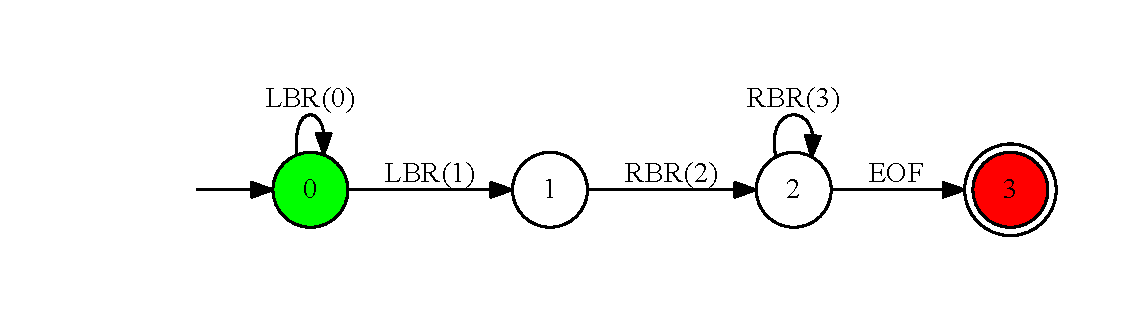
\includegraphics[width=0.38\textwidth]{part_03_GraphAnalysis/chapter_12_CFPQ/figures/07_GLR_Based/input_automaton.pdf}
    \caption{Входной граф-автомат для примера обобщённого RNGLR-алгоритма}
    \label{fig:CFPQ_GLR_input_automaton}
\end{figure}

\mytodo{Перевести обозначения на рисунке.}

Результирующий SPPF показан на рисунке~\ref{fig:CFPQ_GLR_result_sppf}.
Красным отмечены узлы, соответствующие нетерминалу $s$ для распознанных фрагментов входного графа.
Так как вход является графом, SPPF может содержать циклические зависимости и тем самым задавать потенциально бесконечное семейство деревьев вывода конечным образом.

\begin{figure}
    \centering
    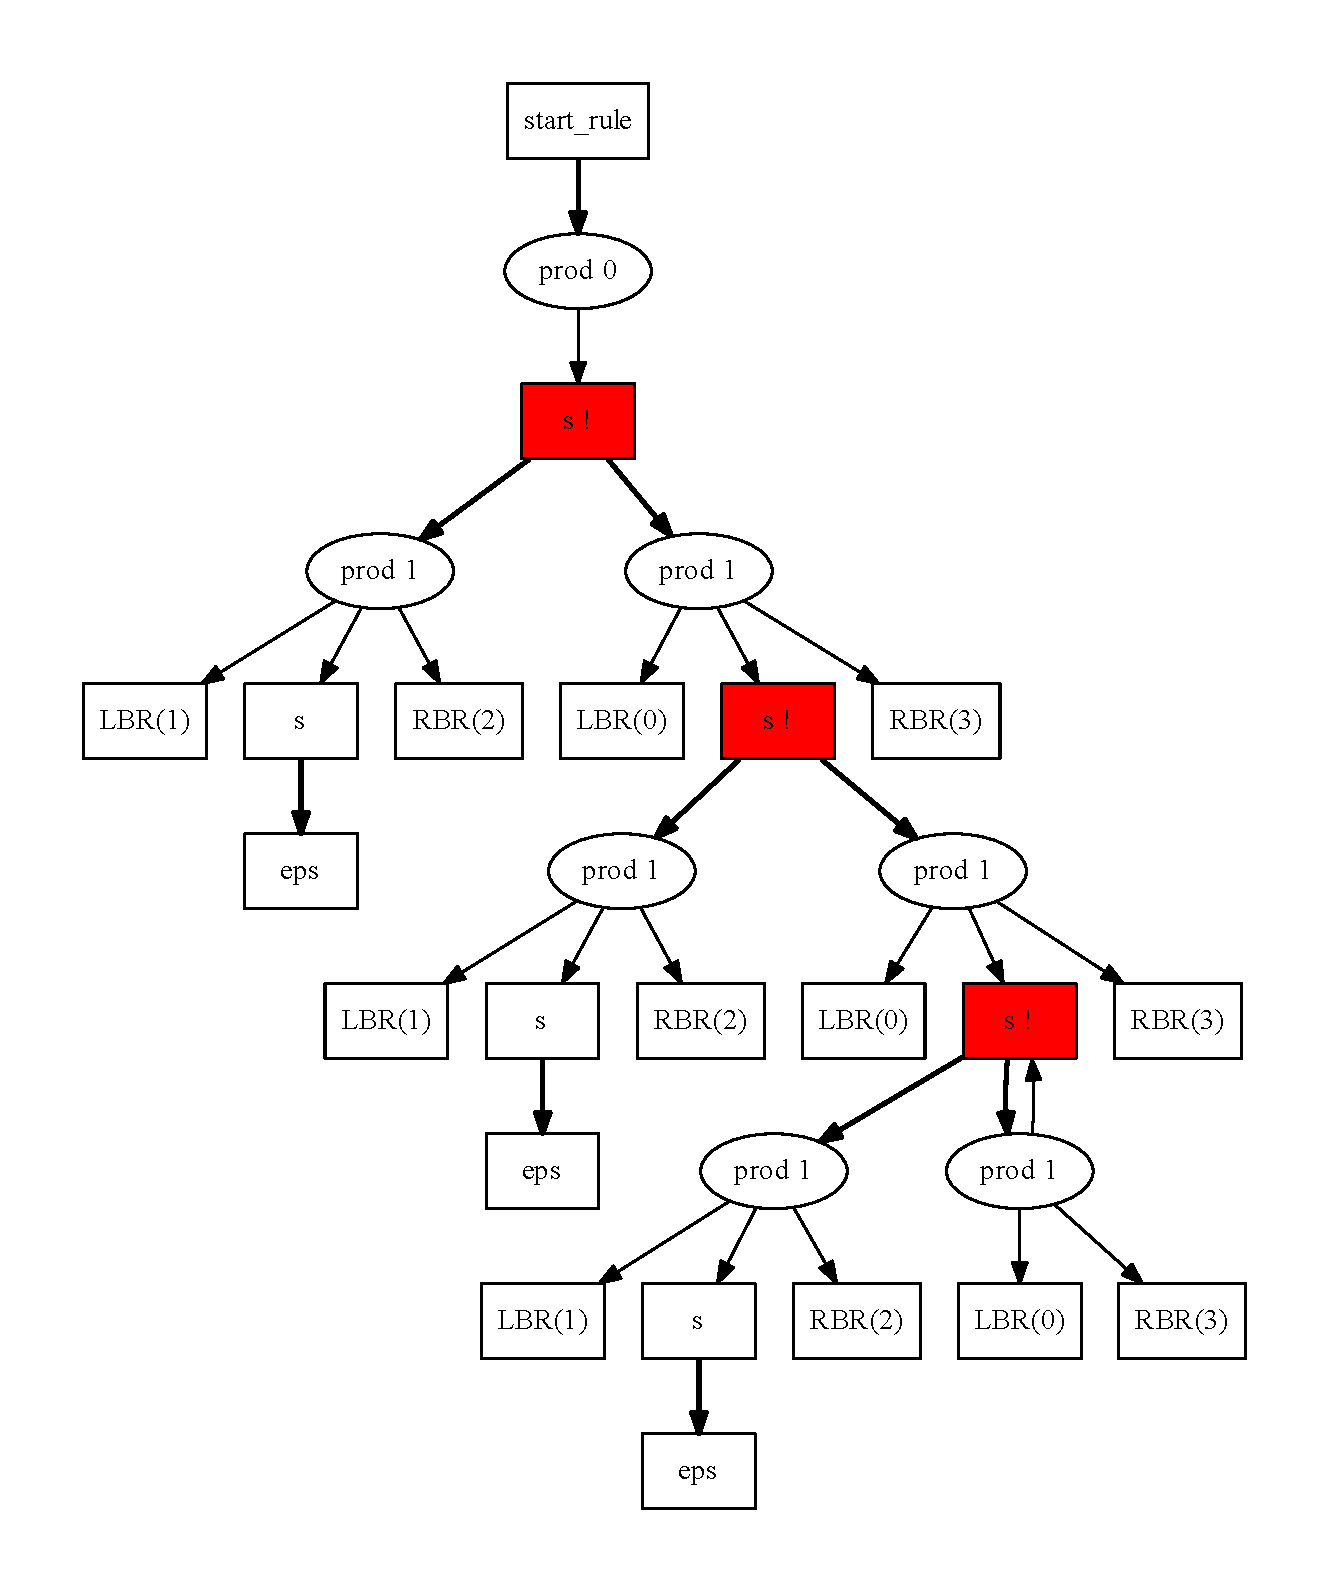
\includegraphics[width=0.72\textwidth]{part_03_GraphAnalysis/chapter_12_CFPQ/figures/07_GLR_Based/result_sppf.pdf}
    \caption{SPPF, построенный обобщённым RNGLR-алгоритмом для графа на рисунке~\ref{fig:CFPQ_GLR_input_automaton}}
    \label{fig:CFPQ_GLR_result_sppf}
\end{figure}

\mytodo{Перевести обозначения на рисунке.}

\subsection{Формальные свойства и доказательства}
\label{subsec:CFPQ_GLR_properties}
\tikzsetfigurename{CFPQ_GLR_Properties_}

\begin{theorem}[Завершимость]
    Алгоритм~\ref{algo:CFPQ_GLR_main} завершается для любого конечного входного графа и любой фиксированной КС-грамматики.
\end{theorem}

\begin{proof}
    Пусть $R$~--- множество состояний RNGLR-анализатора, а $V$~--- множество вершин входного графа.
    В каждой вершине графа может быть создано не более $|R|$ GSS-вершин, поэтому всего GSS содержит не более $|R| \cdot |V|$ вершин.
    Кратные рёбра в GSS не создаются, следовательно, число рёбер GSS конечно и ограничено квадратом числа его вершин.
    Вершины входного графа добавляются в очередь обработки только при добавлении нового ребра GSS или новой задачи, связанной с таким ребром.
    Так как число возможных GSS-рёбер конечно, основной цикл не может выполняться бесконечно.
\end{proof}

Для доказательства корректности используется понятие корректного дерева вывода для входного графа.
Такое дерево имеет стартовый нетерминал грамматики в корне, нетерминалы во внутренних узлах и терминалы в листьях, причём последовательность терминальных листьев соответствует меткам некоторого пути во входном графе.

\begin{lemma}
    Для каждого ребра GSS, связанного с узлом SPPF, терминальные листья соответствующего поддерева задают слово некоторого пути во входном графе.
\end{lemma}

\begin{proof}
    Доказательство проводится индукцией по высоте дерева вывода.
    База соответствует либо $\varepsilon$-дереву, либо дереву из одного терминала.
    В первом случае путь имеет длину ноль, во втором терминал прочитан с некоторого ребра входного графа.
    Для индукционного перехода рассмотрим дерево, корень которого помечен нетерминалом $A$, а дети соответствуют правой части некоторого правила $A \to X_1 \dots X_k$.
    По предположению индукции каждое поддерево $X_i$ соответствует некоторому пути во входном графе.
    Так как эти поддеревья получены одной свёрткой вдоль пути в GSS, конец пути для $X_i$ совпадает с началом пути для $X_{i+1}$.
    Следовательно, их конкатенация задаёт путь во входном графе для всего дерева.
\end{proof}

\begin{theorem}[Звуковость]
    Каждое дерево, восстанавливаемое из построенного SPPF, является корректным деревом вывода для некоторого пути во входном графе.
\end{theorem}

\begin{proof}
    Структура узлов SPPF гарантирует, что внутренние узлы соответствуют нетерминалам грамматики, а продукционные узлы~--- правилам грамматики.
    Остаётся проверить соответствие терминальных листьев пути во входном графе.
    Это следует из предыдущей леммы для GSS-рёбер, из которых формируется результирующий SPPF для принимающих состояний в финальных вершинах графа.
\end{proof}

\begin{theorem}[Полнота]
    Для каждого пути во входном графе, слово которого выводимо из стартового нетерминала грамматики, построенный SPPF содержит соответствующее дерево вывода.
\end{theorem}

\begin{proof}
    Доказательство повторяет доказательство полноты RNGLR для строки, за исключением одного места.
    В классическом RNGLR GSS строится послойно по позициям входной строки: к моменту обработки позиции $i$ все предыдущие уровни уже зафиксированы.
    В графе это свойство нарушается, поскольку новое ребро может появиться в уже существующей части GSS и открыть новый путь для свёртки, которая ранее уже была применена.
    Алгоритм сохраняет проходящие свёртки в вершинах GSS и при добавлении нового ребра продолжает все свёртки, которые должны пройти через это ребро.
    Поэтому ни один путь GSS, соответствующий корректному дереву вывода для пути входного графа, не теряется, а значит соответствующее дерево будет представлено в SPPF.
\end{proof}

Точная асимптотическая оценка времени работы обобщённого алгоритма зависит от способа поиска путей в GSS при свёртках, от числа повторных обработок проходящих свёрток и от размера строящегося SPPF.
В исходной работе подчёркивается, что полная оценка сложности требует отдельного анализа.
Тем не менее из доказательства завершимости следует конечная верхняя граница на число GSS-вершин и GSS-рёбер: при $|R|$ состояниях анализатора и $|V|$ вершинах входного графа число GSS-вершин не превосходит $|R| \cdot |V|$, а число GSS-рёбер~--- $O((|R| \cdot |V|)^2)$.
Если требуется только факт существования пути, можно остановиться после обнаружения принимающей GSS-вершины в финальной вершине графа; если требуется представление всех путей, необходимо построить и сохранить соответствующий SPPF.

\section{Комбинаторы парсеров для поиска путей с КС ограничениям}
	\tikzsetfigurename{CFPQ_Combinators_}

Основные сведения о комбинаторах парсеров вынесены в раздел~\ref{sec:Combinators}.
В данном разделе мы рассматриваем применение этой техники для задачи поиска путей с контекстно-свободными ограничениями в графах (определение~\ref{def:FLPQ}).

Использование комбинаторов для CFPQ решает сразу две задачи.
Во-первых, оно обеспечивает прозрачную интеграцию языка запросов в язык общего назначения~\sidecite{Verbitskaia:2018:PCC:3241653.3241655}: запросы являются обычными функциями, и компилятор языка проверяет их корректность статически.
Это устраняет проблемы подходов на основе строкового встраивания предметно-ориентированных языков (string-embedded DSL) и ORM/LINQ, в которых декомпозиция и переиспользование подзапросов затруднены.
Во-вторых, комбинаторы предоставляют естественный механизм композиции запросов и позволяют строить параметризованные шаблоны типовых запросов (например, запросов вида <<same generation>>~\sidecite{CFGonRDF}).

Идея использовать комбинаторы для навигации по графам не нова; первая реализация была предложена в библиотеке Trails~\sidecite{Kroni:2013:PGA:2489837.2489844}.
Однако Trails, как и большинство библиотек комбинаторов парсеров, не поддерживает леворекурсивные грамматики и испытывает трудности при обработке циклов во входном графе.
Библиотека Meerkat~\sidecite{izmaylova2016practical} решает эти проблемы за счёт идей обобщённого LL-алгоритма (GLL)~\sidecite{Scott:2010:GP:1860132.1860320}: мемоизация~\sidecite{Johnson1995memoization} и передача продолжений (continuation-passing style) позволяют обрабатывать произвольные КС-грамматики, включая леворекурсивные и неоднозначные.
На основе Meerkat была построена библиотека комбинаторов для графовых запросов~\sidecite{Verbitskaia:2018:PCC:3241653.3241655}, которая и рассматривается далее.

\subsection{Описание алгоритма}
\label{subsec:CFPQ_Combinators_description}

В основе подхода лежит следующее наблюдение.
Классический синтаксический анализатор обрабатывает линейный вход~--- строку, которую можно рассматривать как линейный ориентированный граф: символы метят рёбра между соседними позициями.
Анализатор перемещает указатель с позиции $i$ на позицию $i+1$ и создаёт новое состояние, если токен между позициями $i$ и $i+1$ соответствует правилу грамматики.
При переходе к графу общего вида из текущей вершины может исходить несколько рёбер с подходящей меткой, что приводит к порождению нескольких новых состояний.
Обобщённые алгоритмы синтаксического анализа (GLL и GLR) спроектированы для эффективной обработки множественных состояний и потому естественно обобщаются на графы~\sidecite{Grigorev:2017:CPQ:3166094.3166104}.

\subsubsection{Обобщённый интерфейс входа}

Ключевая идея предлагаемого подхода~--- абстрагирование от конкретного представления графа.
Для работы комбинаторов достаточно двух операций, образующих интерфейс \texttt{Input} с параметрами типов меток рёбер $L$ и меток вершин $N$:
\begin{itemize}
    \item \texttt{filterEdges} — по заданной вершине и предикату на метках рёбер возвращает множество исходящих рёбер (метка и целевая вершина);
    \item \texttt{checkNode}~--- проверяет, удовлетворяет ли заданная вершина предикату, и возвращает её метку.
\end{itemize}
Благодаря такому интерфейсу библиотека комбинаторов не зависит от источника данных.
Поддерживаются графы, загруженные в оперативную память, графовая база данных Neo4j и даже линейный вход (обычные строки).

\subsubsection{Базовые комбинаторы}

Библиотека предоставляет набор примитивных комбинаторов и операций для построения более сложных запросов.
Два базовых строительных блока~--- комбинаторы для работы с вершинами и рёбрами:
\begin{itemize}
    \item $V(predicate)$~--- проверяет, что текущая вершина удовлетворяет предикату $predicate$;
    \item $E(predicate)$~--- проверяет, что из текущей вершины исходит ребро, метка которого удовлетворяет предикату $predicate$.
\end{itemize}

На основе этих примитивов строятся более сложные запросы с помощью операций, перечисленных в таблице~\ref{table:CFPQ_Combinators}.
Макрос \texttt{syn} (от \emph{syntax}) преобразует строковый литерал или композицию комбинаторов в рекурсивный нетерминал; например, запись \texttt{val S = syn("a" $\sim$ S.? $\sim$ "b")} задаёт язык $\{a^n b^n \mid n \geq 1\}$.

\begin{table}[h]
    \centering
    \caption{Основные комбинаторы}
    \label{table:CFPQ_Combinators}
    \begin{tabular}{l|l}
        \hline
        Комбинатор & Описание \\
        \hline
        $a \sim b$  & последовательное применение $a$, затем $b$ \\
        $a \mid b$  & альтернатива: $a$ или $b$ \\
        $a?$        & опциональный парсер: $a$ или ничего \\
        $a*$        & повторение нуль или более раз \\
        $a+$        & повторение один или более раз \\
        $a \mathbin{\texttt{\textasciicircum}} f$ & применить функцию $f$ к результату токена $a$ \\
        $a \mathbin{\texttt{\&}} f$ & применить функцию $f$ к результату композиции $a$ \\
        \hline
    \end{tabular}
\end{table}

\subsubsection{Семантические действия}

Для извлечения данных из результатов запроса библиотека предоставляет механизм семантических действий~--- аналог семантических действий в классических генераторах парсеров.
Различают две разновидности:

\begin{itemize}
    \item \texttt{\textasciicircum} применяется к терминальным комбинаторам ($V$ и $E$) и позволяет извлечь свойства токена (например, имя вершины или длину пути);
    \item \texttt{\&} применяется к композиции комбинаторов и позволяет собрать и обработать результаты подзапросов (например, сформировать пару из начальной и конечной вершины пути).
\end{itemize}

Семантические действия вычисляются снизу вверх по дереву разбора (SPPF): сначала обрабатываются действия для дочерних узлов, затем их результаты передаются в действие текущего узла.
Поскольку SPPF может содержать неоднозначные узлы (соответствующие нескольким различным путям), библиотека предоставляет механизм ленивого обхода SPPF в ширину для извлечения деревьев разбора.

Функция \texttt{executeQuery} запускает разбор входного графа из всех вершин, строит SPPF, извлекает все деревья разбора, применяет семантические действия и возвращает ленивый поток результатов.

\subsubsection{SPPF как представление результата}

В основе библиотеки Meerkat лежит обобщённый LL-алгоритм, который строит сжатое представление леса разбора~--- SPPF (раздел~\ref{sec:GLR}).
Как было показано ранее~\sidecite{Grigorev:2017:CPQ:3166094.3166104}, SPPF является подходящим конечным представлением потенциально бесконечного множества путей.
Все пути могут быть извлечены из SPPF в виде соответствующих деревьев вывода.

\subsubsection{Обработка циклов и левой рекурсии}

Мемоизация, используемая в Meerkat, решает две ключевые проблемы, возникающие при обработке графов.
Во-первых, разбор из заданного состояния в заданной вершине выполняется только один раз; поскольку число состояний и вершин конечно, разбор гарантированно завершается, и бесконечные циклы при обходе циклов графа невозможны.
Во-вторых, появление нового состояния разбора в вершине, которая уже была обработана, запускает пересчёт всех зависимых от него путей.
Благодаря мемоизации каждый вывод каждого подпути анализируется ровно один раз, что не приводит к существенным накладным расходам.

Этот же механизм мемоизации и передачи продолжений (continuation-passing style) позволяет Meerkat обрабатывать леворекурсивные комбинаторы~\sidecite{izmaylova2016practical}, что является общей проблемой подхода комбинаторов парсеров.

\subsection{Примеры}
\label{subsec:CFPQ_Combinators_examples}

\subsubsection{Запрос same generation}

Рассмотрим классический контекстно-свободный запрос <<same generation>>~\sidecite{CFGonRDF}, полезный для анализа иерархий в RDF-графах.
Пусть граф содержит отношения двух типов: \texttt{subClassOf} и \texttt{type}, а также обратные к ним \texttt{subClassOf}$^{-1}$ и \texttt{type}$^{-1}$.
Задача~--- найти вершины, находящиеся на одном уровне иерархии, то есть достижимые путями, в которых каждому шагу <<вверх>> соответствует шаг <<вниз>> по парному отношению.

Грамматика для этого запроса на двух парах отношений имеет вид:
\[
    \mathit{qSameGen} \to \mathit{R}_0^{-1}\ \mathit{qSameGen?}\ \mathit{R}_0 \mid \mathit{R}_1^{-1}\ \mathit{qSameGen?}\ \mathit{R}_1
\]
где $\mathit{R}_0 = \text{\texttt{subClassOf}}$, $\mathit{R}_1 = \text{\texttt{type}}$, а $\mathit{R}_i^{-1}$ обозначает обратное отношение.
Средствами комбинаторов этот запрос записывается следующим образом:

\begin{verbatim}
val qSameGen = syn(
    inE(_.label == "subClassOf") ~ qSameGen.? ~ outE(_.label == "subClassOf") |
    inE(_.label == "type") ~ qSameGen.? ~ outE(_.label == "type"))
\end{verbatim}

% TODO: Здесь было бы хорошо привести рисунок графа, на котором демонстрируется запрос.
% \mytodo{Создать рисунок графа для примера same generation.}

\subsubsection{Параметризованные комбинаторы и композиция}

Грамматики для запросов <<same generation>> над разными наборами пар отношений структурно идентичны и различаются лишь конкретными отношениями.
Средствами комбинаторов это обобщение выражается естественно: функция \texttt{sameGen} принимает список пар <<скобок>> и строит соответствующий запрос.

Вспомогательная функция \texttt{reduceChoice} сводит список подзапросов к одному с помощью операции альтернативы:

\begin{verbatim}
def reduceChoice(qs: List[Nonterminal]) = qs match {
    case x :: Nil => x
    case x :: y :: qs => syn(qs.foldLeft(x | y)(_ | _))
}
\end{verbatim}

Тогда параметризованный комбинатор \texttt{sameGen} определяется как:

\begin{verbatim}
def sameGen(brs: List[(Nonterminal, Nonterminal)]) =
    reduceChoice(brs.map { case (lbr, rbr) =>
        syn(lbr ~ sameGen(brs).? ~ rbr) })
\end{verbatim}

Теперь запросы над разными наборами отношений конструируются простым применением \texttt{sameGen} к нужному списку пар, без дублирования кода.

\subsubsection{Семантические действия и типобезопасность}

Продолжим пример запроса <<same generation>>.
Пусть требуется не только найти достижимые вершины, но и вычислить длину каждого пути.
Добавим семантические действия для аккумулирования длины:

\begin{verbatim}
def sameGen(brs: List[(_, _)]) =
    reduceChoice(brs.map { case (lbr, rbr) =>
        syn((lbr ~ (sameGen(brs).?) ~ rbr) & {
            case _ ~ Nil ~ _       => 2
            case _ ~ (len: Int) ~ _ => len + 2
        })
    })
\end{verbatim}

Здесь \texttt{\&} применяется к результату последовательности из трёх элементов.
Если средний элемент отсутствует (путь нулевой длины между <<скобками>>), длина пары скобок равна 2; иначе к накопленной длине добавляются два ребра текущей пары.

Поскольку запросы являются обычными функциями языка Scala, компилятор статически проверяет корректность типов.
Например, если в семантическом действии вместо целого числа попытаться использовать строку, компилятор укажет на ошибку типа.
Кроме того, IDE предоставляет подсветку синтаксиса, навигацию по коду и автодополнение без дополнительных настроек.

\begin{example}
    Рассмотрим запрос к онтологии \emph{Geospecies}, содержащей биологическую иерархию.
    Для стартовой вершины $v$ запрос на основе комбинатора \texttt{sameGen} с отношением \texttt{skos\_\_narrowerTransitive} возвращает множество объектов одного уровня иерархии.
    Одновременно вычисляется длина соответствующих путей.
    Эксперименты на реальных RDF-графах показывают, что время выполнения и потребление памяти линейны по размеру результирующего множества путей.
\end{example}

\subsection{Свойства алгоритма}
\label{subsec:CFPQ_Combinators_properties}

Опишем основные свойства подхода.

\begin{theorem}[Корректность]
    Множество путей, построенное библиотекой комбинаторов для запроса, заданного КС-грамматикой $G$ и графа $\mbfscrG$, совпадает с множеством путей задачи CFPQ для $G$ и $\mbfscrG$.
\end{theorem}

\begin{proof}
    Корректность следует из корректности GLL-алгоритма~\sidecite{Scott:2010:GP:1860132.1860320} и его обобщения на графы~\sidecite{Grigorev:2017:CPQ:3166094.3166104}.
    Библиотека Meerkat реализует обобщённый LL-алгоритм, а обобщение на графы достигается заменой функции перехода <<следующая позиция>> на функцию \texttt{filterEdges}, возвращающую множество следующих вершин.
    Корректность этого обобщения показана в~\sidecite{Verbitskaia:2018:PCC:3241653.3241655}.
\end{proof}

\noindent\textbf{Выразительная мощность.}
Подход поддерживает произвольные КС-грамматики, включая леворекурсивные и неоднозначные.
Это обеспечивается мемоизацией и передачей продолжений~\sidecite{izmaylova2016practical,Johnson1995memoization}.

\medskip
\noindent\textbf{Обработка циклов.}
Мемоизация гарантирует завершение разбора на графах с циклами: каждое состояние разбора в каждой вершине обрабатывается не более одного раза, а число состояний конечно.

\medskip
\noindent\textbf{Сложность.}
В худшем случае временная и пространственная сложность кубические относительно размера графа, что унаследовано от GLL-алгоритма~\sidecite{Scott:2010:GP:1860132.1860320}.
На практике для задачи с одним источником (single-source CFPQ) время выполнения часто линейно по размеру результата, что подтверждается экспериментальными данными~\sidecite{Verbitskaia:2018:PCC:3241653.3241655}.

\medskip
\noindent\textbf{Представление результата.}
SPPF (раздел~\ref{sec:GLR}) является конечной структурой данных, представляющей потенциально бесконечное множество путей.
Из SPPF могут быть лениво извлечены все деревья вывода с применением семантических действий.

\medskip
\noindent\textbf{Сравнение с другими подходами.}
В отличие от матричных алгоритмов (раздел~\ref{sec:MatrixCFPQ}), вычисляющих достижимость между всеми парами вершин, комбинаторы естественно поддерживают семантику с одним источником и не требуют приведения грамматики к нормальной форме Хомского, как подходы на основе CYK (раздел~\ref{sec:CYK}), GLL (раздел~\ref{sec:CFPQ_GLL}) и GLR (раздел~\ref{sec:GLR}).
Дополнительным преимуществом является возможность задания пользовательских семантических действий и параметризованных шаблонов запросов, обеспечиваемая интеграцией в язык общего назначения.

